\chapter{System Analysis and Design\label{ch:System Analysis and Design}}

\section{Use Case}
\begin{tikzpicture}  

\begin{umlsystem}[x=0, fill=red!8]{Real Time Pakistani Sign language Recognition Using Kinect} 


\umlusecase[y=-1]{Get a Sign}  \umlusecase[y=-3]{Translate the Sign}  
\umlusecase[y=-5]{Record the sign}   \end{umlsystem}   

\umlactor[x=-7.5,y=-3]{listener} \umlactor[x=7,y=-2]{kinect}  \umlactor[x=7,y=-5]{Storage}   


\umlassoc{listener}{usecase-1}  \umlassoc{listener}{usecase-1}  \umlassoc{kinect}{usecase-1}  \umlassoc{listener}{usecase-2} 

\umlassoc{Storage}{usecase-3}   

\umlassoc{listener}{usecase-3} 

\umlassoc{Storage}{usecase-3} 

\end{tikzpicture}

Where the color spectrum from black to brighter gray represents the primary, secondary and outstanding actors
\clearpage
\section{Get the sign}
\begin{table}[htbp]
	\centering
	
	\caption{Get the Sign}
	
	\begin{tabular}{|p{3cm}|p{11cm}| } 
		\hline
		
		 Id &  1  \\ 
		\hline
		 Title &  Get Sign  \\ 
		\hline
		 Description &  Start getting the sign to be translated from the Kinect device.  \\ 
		\hline
		 Actor & Listener \\
		\hline
		 Pre-Condition & System must be 'On'.  \\ 
		\hline
		 Post Condition &  Frames of sign are being received live from Kinect Camera by the software. \\ 
		\hline
		 Success Scenario &  Learning module receives frames from the Kinect Device.  \\ 
		\hline
		 Alternative Flow &  Corresponding error displayed to user and program aborts.  \\ 
		\hline
		 Stakeholders &  Listener(operator), Signer.  \\ 
		\hline
	     Special Requirements &  Kinect must be powered, Kinect is successfully connected to the system.
		\\ 
		\hline
		 Open Issues &  The system when gets the sign then it stores the sign in an excel file. This file sometimes gets corrupted because of some internal file system error. \\ 
		\hline
	\end{tabular}  
	\clearpage        
\end{table}
A user arrives on the interface terminal. System presents him with three buttons labelled as ‘start’, ‘end’ and ‘Predict’. If user wants to get the sign recorded from the Kinect, he would press the ‘start’ button. The system has now started recording the sign. As the sign duration ends, the user has to press the ‘end’ button. As the ‘end’ button is pressed, sign is saved in the directory and can be used for further operations.

\clearpage
\subsection{Translate the sign}
\begin{table}[htbp]
	\centering
	
	\caption{Translate the sign}
	\begin{tabular}{ |p{3cm}|p{11cm}| } 
		\hline
		 Id &  2  \\ 
		\hline
		 Title &  Translate the sign  \\ 
		\hline
		 Description &  Sign is being received in form of series of frames from the Kinect Camera. Now this sign needs to be translated if Listener opts to translate.  \\ 
		\hline
		 Actor & Listener \\
		\hline
		 Pre-Condition & Program started receiving frames from the Kinect in form of series of frames.  \\ 
		\hline
		 Post Condition & Sign is evaluated and processed by the system and translated to a label or voice chunk. \\ 
		\hline
		 Success Scenario &  Sign is translated to a right label or voice chunk.  \\ 
		\hline
		 Alternative Flow &  Sign is translated to a wrong label or voice chunk.  \\ 
		\hline
		 Stakeholders &  Listener(operator).   \\ 
		\hline
		 Special Requirements &  Kinect must be powered, Kinect is successfully connected to the system,Sign must be recorded and stored successfully.  \\ 
		\hline
		 Open Issues & A naïve sign if done would be predicted to the class closest in features. So validity is only ensured if a sign is done from the predefined sentences. \\ 
		\hline
	\end{tabular}   
	
\end{table}
The signer has recorded the sign using the 'start' and 'end' button. Now he presses the 'predict' button. As he presses the button the system looks for the sign in the corresponding directory and then predicts it against the model. The 'label' is presented to the signer in the lower right text box. 

\clearpage
\subsection{Save the Sign}
\begin{table}[htbp]
	\centering
	\caption{Save the Sign}
	\begin{tabular}{ |p{3cm}|p{11cm}| } 
		\hline
		 Id &  3  \\ 
		\hline
		 Title &  Save the Sign  \\ 
		\hline
		 Description &  Sign can be saved to some repository and can be translated later if wanted.  \\ 
		\hline
		 Actor & Listener \\
		\hline
		 Pre-Condition & System must be 'On'.  \\ 
		\hline
		 Post Condition &  A sign is saved in form of a video to a repository. \\ 
		\hline
		 Success Scenario &  Sign was saved to repository.  \\ 
		\hline
		 Alternative Flow &  Corresponding error to user and system rolled back to previous safe point.  \\ 
		\hline
		 Stakeholders &  Listener(operator)  \\ 
		\hline
		 Special Requirements &  Kinect must be powered,
		Kinect is successfully connected to the system,
		All the libraries are successfully imported. \\ 
		\hline
		 Open Issues &  Note that only one sign can be saved for the future work not more than one.  \\ 
		\hline
	\end{tabular}   
	
\end{table}
The operator will record the sign using the 'start' and 'end' button. Now the operator presses the 'start' button
the data will be start storing when the operator clicks on 'end' button, the storage of the sign will be stopped.   

\clearpage
\section{Flow Diagram}
\begin{figure}[!h]
	\begin{center}
		
		\tikzstyle{decision} = [diamond, draw, fill=blue!20, 
		text width=4.5em, text badly centered, node distance=3cm, inner sep=0pt]
		\tikzstyle{block} = [rectangle, draw, fill=blue!20, 
		text width=6em, text centered, rounded corners, minimum height=4em]
		\tikzstyle{line} = [draw, -latex']
		\tikzstyle{cloud} = [draw, ellipse,fill=red!20, node distance=3cm,
		minimum height=2em]
		
		\begin{tikzpicture}[node distance = 3cm, auto]
		% Place nodes
		
		\node [block] (init) {Input Sign};
		
		\node [block, below of=init] (identify) {Segmentation };
		
		\node [block, below of=identify] (evaluate) {Time Series \\ Feature};
		
		\node [block, left of=evaluate, node distance=5cm] (update) {Time Series \\ Generation};
		
		\node [decision, below of=evaluate] (decide) {Model};
		
		\node [block, below of=decide, node distance=3.5cm] (stop) {Sign Label};
		
		
		\node [block, above of=update] (system2) {Feature \\ Extraction};
		
		\node [block, above of=system2] (system3) {Input Sign};    
		
		
		
		% Draw edges
		\path [line] (init) -- (identify);
		
		
		\path [line] (identify) -- (evaluate);
		\path [line] (evaluate) -- node {Testing} (decide);
		
		\path [line] (system3) -- (system2);
		
		\path [line] (system2) -- (update);
		
		\path [line] (update) |- node [near start] {Training} (decide);
		
		\path [line] (decide) -- (stop);
		
		
		\end{tikzpicture}
		
	\end{center}
\end{figure}



\clearpage
\section{System Sequence Diagram}

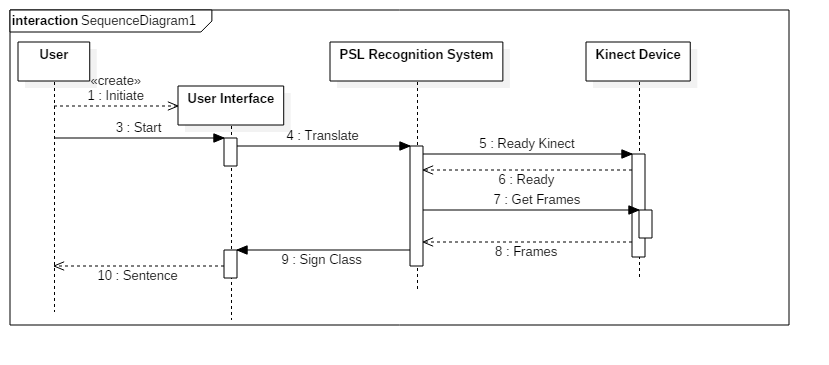
\includegraphics[height=10cm, width=17cm]{ThesisFigs/sequencediagram}

